\chapter{Turvallisuus\label{Turvallisuus}}

Kaksi- ja monivaiheisten kirjautumismenetelmien on todettu tuovan parempaa turvaa kuin yksivaiheinen kirjautuminen. Kaksi- ja monivaiheisten kirjautumismenetelmien suojaavat käyttäjätilien joutumista vääriin käsiin automaattisia hyökkäyksissä, kalasteluhyökkäyksissä sekä kohdennetuissa hyökkäyksissä. Vaikka kaksi- ja monivaiheinen kirjautuminen tuovat parempaa turvaa ja suojaavat käyttäjätilejä paremmin liittyy näihinkin menetelmiin turvallisuusriskejä. Seuraavaksi tutkimme millaisia turvallisuusriskejä ja ongelmia varmentamismenetelmiin liity. 

Turvallisuus riskit voidaan jakaa kolmeen kategoriaan perustuen samoihin kategorioihin kuin todentamistavoissa. Ensimmäisenä haavoittuvana ja vaarantuneena tekijänä on jotain mitä tiedät. Hyökkääjä voi arvata salaisuuden, jonka tiedät käyttämällä esimerkiksi arvaamalla käyttäen raakaa voimaa. Vuotaneet käyttäjätunnukset ja salasanat ovat myös turvallisuus riski. Ihmiset käyttävät samoja tai samanlaisia salasanoja useissa palveluissa. Hyökkääjä voi käyttää vuotaneita salasanoja hyväkseen. Haittaohjelmat ovat myös turvallisuus riski. Haittaohjelma voi varastaa tietokoneelle tallennetut käyttäjätunnukset. Haittaohjelma pystyy myös seuraamaan käyttäjän näppäimistösyötteitä ja tätä kautta saada salasana varastettua. Myös yksinkertaiseen asiaa kuin salasanan kirjoittamiseen paperille liittyy turvallisuusriski. Tämä paperi voi hävitä tai se voidaan varastaa.

Seuraava turvallisuus riski liittyy asioihin, joita omistat. Jotain mitä omistat asioita ovat esimerkiksi puhelin, fyysinen avain tai käyntikortti. Jotain mitä omistat voi hävitä tai hajota. Hyökkääjä voi myös varastaa tai kloonata esineen tai laitteen. Viruksen tai haittaohjelman avulla hyökkääjä voi saada pääsyn esimerkiksi puhelimessa olevaan varmentamisohjelmaan. 

Viimeiseksi turvallisuuteen kohdistuvat ongelma liittyvät jotain mitä olet kategoriaan. Jotain mitä olet ihmisten yksilöllisiä asioita kuten kasvot, sormenjälki ja ääni. Nämä ovat yksilöllisiä asioita ja niiden kopiointi tai manipulointi on haastavaa.

NIST (National Institute of Standards and Technology) on määritellyt esimerkkejä kirjautumisiin liittyvistä turvallisuus riskeistä sekä mahdollisia menetelmiä näiden korjaamiseen. Kirjautumismenetelmiin liittyviä turvallisuus riskejä on runsaasti, eikä kaikkia pystytä käymään yksitellen läpi. Tutkittavaksi turvallisuusriskeiksi on valittu SMS varmenteeseen sekä TOTP:hen liittyviä turvallisuusriskejä. \citep{NIST_800_63B}



\section{SMS varmenne}
\begin{figure}[ht]
    \centering
    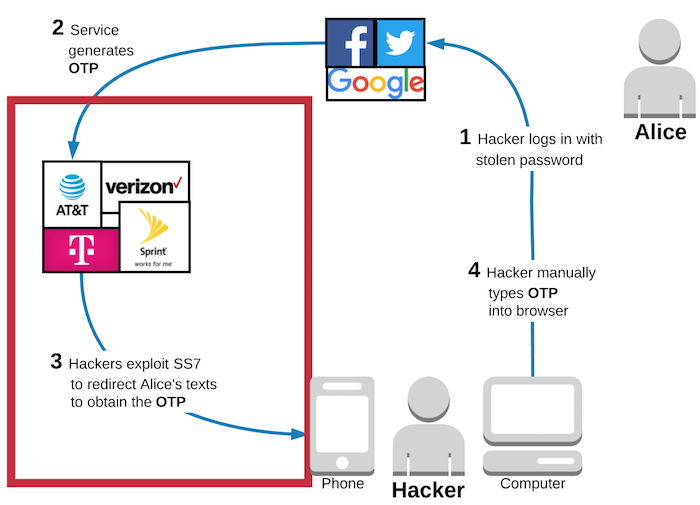
\includegraphics[width=10cm]{template/figures/SS7 attack vulnerable.png}
    \caption{SS7 haavoittuvuus SMS varmentamisessa \citep{2FA_SMS}}
    \label{fig:ss7SMSM}
\end{figure}

SS7 on lyhenne sanoista \emph{Signaling System 7} on vuonna 1975 kehitetty joukko puhelinliikenteen signalointiprotokollille. SS7 protokolaa käytetään puheluiden muodostamiseen, puhelinnumeroiden kääntämiseen ja siirtämiseen, SMS viestien lähettämiseen ja muihin palveluihin. SS7 on vanha systeemi ja siihen liittyy monia havaittuja ja käytettyjä turvallisuusriskejä. Ensimmäinen turvallisuus riski liittyy käyttäjien seuraamiseen. SS7 avulla on mahdollista seurata käyttäjän puhelimen liikkumista missä tahansa maailmaa noin 70 \% tarkkuudella. Toinen turvallisuus riski liittyy puheluiden ja viestien kaappaamiseen. Puheluita ja viestejä on mahdollista siirtää toiseen puhelimeen. Hyökkääjät voivat käyttää näitä menetelmiä hyväkseen. \citep{ss7} 

Kuva \ref{fig:ss7SMSM} havainnollistaa kaksivaiheisen kirjautumisen toimintaa, jossa käytetään salasanaa ja tekstiviestillä lähetettävää vahvistuskoodia varmentamiseen. Ensimmäiseksi hyökkääjä kirjautuu varastetuilla tunnuksilla palveluun. Tämän jälkeen palvelu tunnistaa, että käyttäjällä on kaksivaiheinen tunnistautuminen käytössä. Palvelu luo kertakäyttöisen koodin ja lähettää sen tekstiviestinä. Tämän jälkeen siirrytään kuvan \ref{fig:ss7SMSM}  kolmanteen vaiheeseen, joka on merkitty punaisella kehyksellä. Kolmannessa vaiheessa hyökkääjä käyttää SS7 järjestelmään tunnettuja haavoittuvuuksia hyväkseen. Hyökkääjä hyödyntää haavoittuvuuksia kertakäyttöisenkoodin saamiseksi. Saatuaan kertakäyttöisenkoodin hyökkääjä syöttää saadun kertakäyttöisenkoodin ja saa pääsyn käyttäjätilille. 


\section{TOTP}

Kaksivaiheiseen kirjautumiseen, jossa käytetään TOTP:tä liittyy muutamia turvallisuus Ongelmia.

\begin{figure}[ht]
    \centering
    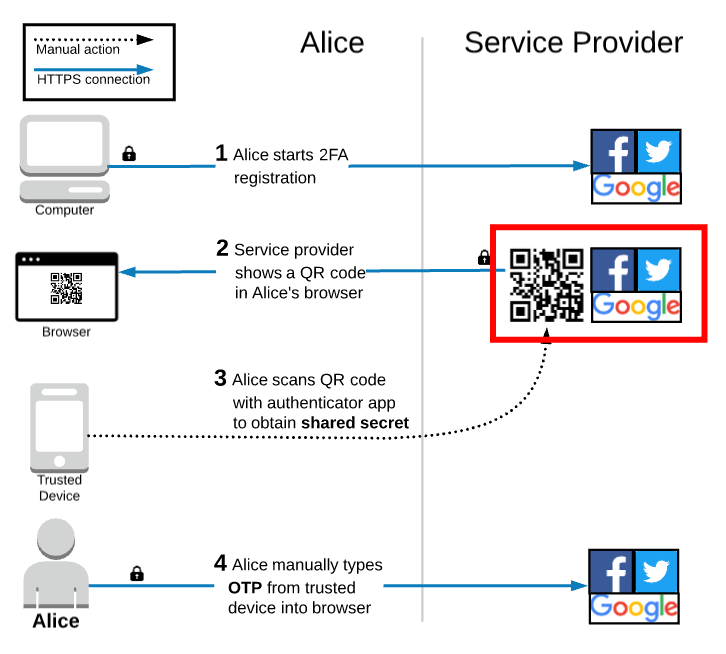
\includegraphics[width=10cm]{template/figures/TOTP service-provider-compromise.png}
    \caption{TOTP salaisen avaimeen turvallisuus ongelma\citep{TOTP}}
    \label{fig:TOTP_service_provider}
\end{figure}

Kuvassa \ref{fig:TOTP_service_provider} on merkattu punaisella ensimmäinen TOTP:n käyttämiseen liittyvä turvallisuus ongelma. TOTP:n toiminta perustuu salaiseen avaimeen, jonka palvelun tarjooja antaa käyttäjälle. Salainen avain näytetään yleensä QR koodi muodossa, jonka pystyy skannaamaan puhelimella. Tähän liittyy turvallisuus riski. Jos hyökkääjä saa salaisen avaimen haltuunsa hänellä on pääsy TOTP:n kertakäyttöisiin koodeihin. Näin kaksivaiheisen kirjautumisen hyöty häviää. 

\begin{figure}
    \centering
    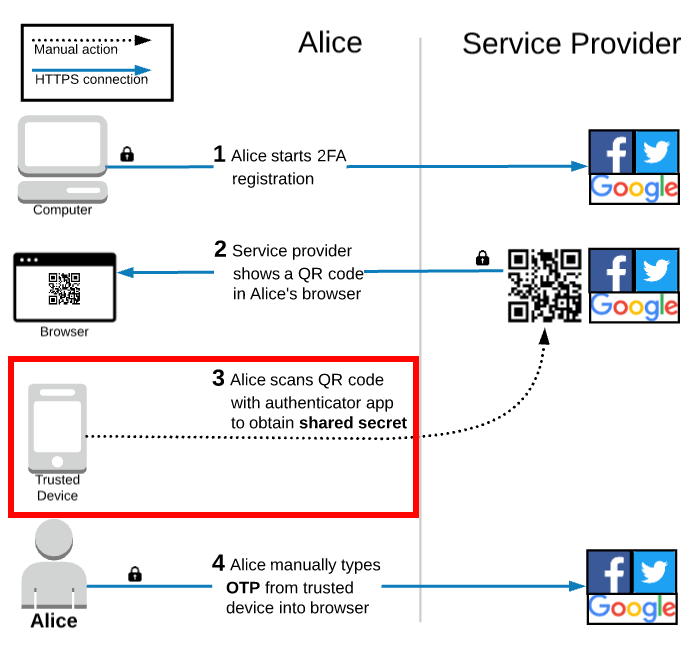
\includegraphics[width=10cm]{template/figures/TOTP trusted-device-compromise.png}
    \caption{TOTP luotetun laitteen turvallisuus ongelma \citep{TOTP}}
    \label{fig:TOTP_device}
\end{figure}

Kaksivaiheisessa kirjautumisessa missä käytetään TOTP:tä salaisten avaimien tallentamiseen käytetään yleensä puhelinta, joka tässä tapauksessa on luotettu laite. Puhelimeen on tallennettu salaiset avaimet, joiden perusteella kertakäyttöiset koodit luodaan. TOTP:n toinen turvallisuus riski liittyy puhelimeen. Kuvassa \ref{fig:TOTP_device} on punaisella merkitty tätä turvallisuus ongelmaa. Puhelinta pidetään luotettuna laitteena ja oletetaan oikean omistajan olevan vain pääsy siihen. Puhelin voi hävitä tai se voidaan varastaa. Myös haittaohjelmat voivat varastaa TOTP salaiset avaimet. 



Teknologien turvallisuus kehittyy ja paranee jatkuvasti. Yksi mittari on verkkosivujen siirtyminen käyttämään HTTPS-protokolaa. HTTPS-protokolan avulla verkkosivujen tiedot siirtyvät salatusti verkossa. Tällä hetkellä 95\% verkkosivuista käyttää HTTPS-protokollaa. Vaikka verkkosivujen turvallisuus on parantunut yksiasia, joka ei ole parantunut ja vähentynyt on kalasteluhyökkäykset. \citep{google_transparency_report} \citep{phishing_scams}

\begin{figure}[ht]
    \centering
    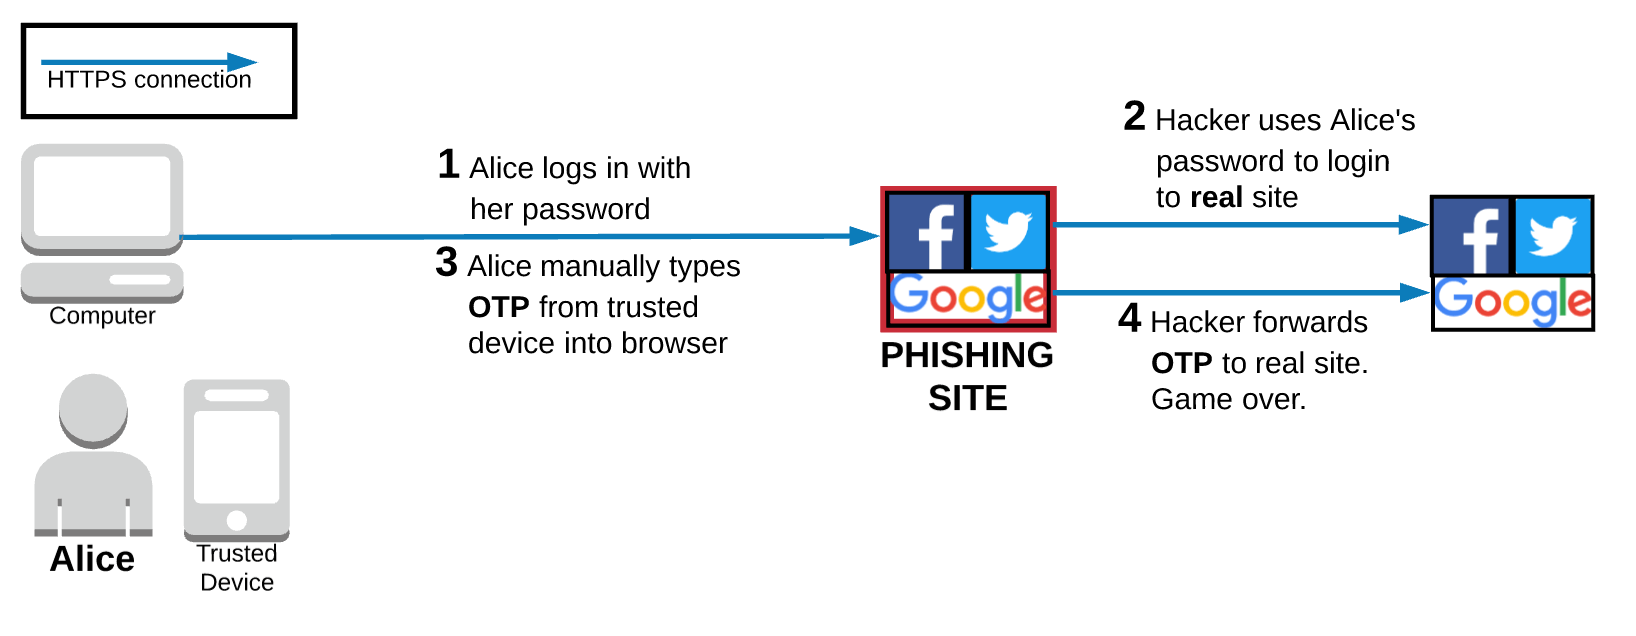
\includegraphics[width=15cm]{template/figures/totp phishing attack.png}
    \caption{TOTP kalasteluhyökkäys \citep{TOTP}}
    \label{fig:TOTP_phishing}
\end{figure}

Kaksivaiheiseen tunnistautumiseen, jossa käytetään TOPT:tä liittyy kalasteluhyökkäyksen riski. Kalastelu hyökkäyksessä hyökkääjä on tehnyt aidon näköisen verkkosivun, jossa pyydetään käyttäjää antamaan käyttäjätietoja. Kalastelusivu voi olla aidon näköinen, joten käyttäjä luulee sivuston olevan aito ja oikea. Kuvassa \ref{fig:TOTP_phishing} on kuvattu kalastelusivun toimintaa. Ensimmäisessä ja kolmannessa kohdassa käyttäjä syöttää salasanan sekä kertakäyttöisen koodi. Käyttäjä luulee kirjautuvansa oikealle sivulle, mutta todellisuudessa käyttäjä syöttää tiedot kalastelusivulle. Kohdissa kaksi ja neljä hyökkääjä hyödyntää käyttäjän kalastelusivulla syöttämiä tietoja ja kirjautuu oikeaan palveluun. Näin hyökkääjä saa pääsyn käyttäjätilille. Vaikka kaksivaiheinen kirjautuminen oli käytössä ei se estä kalastelusivuihin liittyvää turvallisuusongelmaa. 

Kuva \ref{fig:TOTP_phishing} kuvasi mahdollisen kalasteluhyökkäyksen toimintaa. Kalasteluhyökkäyksiä voidaan toteuttaa muillakin tavoilla. SMS varmenne on myös haavoittuvainen kalasteluhyökkäykselle. SMS varmentamisessa lähetetään kertakäyttöinen koodi tekstiviestinä käyttäjän puhelimeen. Hyökkääjä tarvitsee tämän koodin kirjautumista varten. Hyökkääjä voi yrittää kalastella tätä koodia lähettämällä käyttäjälle kalastelu tekstiviestin, jossa pyydetään lähettämään äsken saatu kertakäyttöinen koodi. \citep{google_transparency_report} 

Kalasteluhyökkäyksiä pyritään estämään monilla eri menetelmillä. Mobiilisovellukseen perustuva kaksivaiheinenkirjautuminen on parempi vaihtoehto. Se estää tekstiviesti ja sähköposti kalasteluhyökkäyksiä. Sähköpostipalvelut voivat myös estää kalasteluhyökkäyksiä. Palvelut voivat kehittää menetelmiä, joilla tunnistetaan epäilyttävät ja mahdolliset kalastelu sähköpostit. Käyttäjien myös tulisi itse olla tarkempi mille sivuille kirjautuu. Vaikka kalasteluhyökkäys on edelleen merkittävä ongelma nykyisillä sekä uusilla menetelmillä pyritään kalasteluhyökkäyksiä estämään. \citep{google_transparency_report}  


